%\begin{table}[!t]
\centering
\caption{Performance statistics of \tool}
\label{tab:runtime}
\resizebox{0.48\textwidth}{!}{%
\begin{tabular}{|l|r|r|r|r|r|}
\hline
            \textbf{Case}         & \textbf{Causality} & \textbf{Edge Merge} & \textbf{Node Split} & \textbf{Weight} & \textbf{Rep. Propagation} \\ \hline
penetration-c1       & 0.088                     & 0.001           & 0.002             & 0.013                          & 0.069                              \\ \hline
penetration-c2       & 0.086                     & 0.000           & 0.000             & 0.027                          & 0.001                              \\ \hline
password-crack-c1    & 0.186                     & 0.001           & 0.000             & 0.009                          & 0.000                              \\ \hline
password-crack-c2    & 0.183                     & 0.007           & 0.001             & 0.015                          & 0.001                              \\ \hline
password-crack-c3    & 0.256                     & 0.152           & 0.001             & 0.022                          & 0.000                              \\ \hline
data-leakage         & 0.568                     & 0.450           & 0.019             & 1.697                          & 0.031                              \\ \hline
command-injection-c1 & 0.246                     & 0.001           & 0.001             & 0.020                          & 0.000                              \\ \hline
command-injection-c2 & 0.215                     & 0.025           & 0.006             & 0.668                          & 0.008                              \\ \hline
vpnfilter-c1         & 0.179                     & 0.002           & 0.000             & 0.006                          & 0.000                              \\ \hline
vpnfilter-c2         & 0.162                     & 0.007           & 0.000             & 0.053                          & 0.000                              \\ \hline
\textbf{avg}         & \textbf{0.21}            & \textbf{0.06}  & \textbf{0.003}   & \textbf{0.25}                 & \textbf{0.01}                     \\ \hline
\end{tabular}
}
\end{table}

\begin{table*}[]
\centering
\caption{Runtime performance of \tool and baseline approach}
\resizebox{0.96\textwidth}{!}{
\begin{tabular}{crrrrrr}
\hline

                            & \multicolumn{1}{c}{}                                             & \multicolumn{1}{c}{}                                         & \multicolumn{2}{c}{\textbf{Dependency Weight Computation (s)}}                                      & \multicolumn{2}{c}{\textbf{Dependency Impact Propagation (s)}}                                             \\ \cline{4-7} 

\multirow{-2}{*}{\textbf{Attack}} & \multicolumn{1}{c}{\multirow{-2}{*}{\textbf{Causality Ana.(s)}}} & \multicolumn{1}{c}{\multirow{-2}{*}{\textbf{Edge Merge(s)}}} & \multicolumn{1}{c}{\tool} & \multicolumn{1}{c}{Avg. Proj.} & \multicolumn{1}{c}{\tool} & \multicolumn{1}{c}{Avg. Proj.} \\ \hline
Wget executable                                         & 120.97                                                                                   & 0.05                                                                                 & 0.26                                                & 0.02                                                      & 0.06                                                & 0.06                                                      \\ 

Illegal storage                                         & 92.86                                                                                    & 0.38                                                                                 & 7.43                                                & 0.39                                                      & 19.48                                               & 47.77                                                     \\ 
Illegal storage 2                                       & 95.13                                                                                    & 3.02                                                                                 & 52.68                                               & 33.79                                                     & 160.08                                              & 1,038.55                                                  \\ 

Hide File                                               & 223.63                                                                                   & 42.16                                                                                & 463.68                                              & 16.14                                                     & 1,150.35                                            & 8,486.32                                                  \\ 
Steal Information                                       & 129.82                                                                                   & 39.51                                                                                & 479.02                                              & 15.98                                                     & 1,157.45                                            & 8,128.28                                                  \\ 

Backdoor Download                                       & 19.74                                                                                    & 0.44                                                                                 & 13.87                                               & 0.32                                                      & 12.75                                               & 24.05                                                     \\ 
Annoying Server User                                    & 17.23                                                                                    & 0.01                                                                                 & 0.18                                                & 0.01                                                      & 0.03                                                & 0.03                                                      \\ 

Shellshock                                              & 0.05                                                                                     & 0.03                                                                                 & 0.07                                                & 0.01                                                      & 0.02                                                & 0.06                                                      \\ 
Dataleak                                                & 0.09                                                                                     & 0.01                                                                                 & 0.28                                                & 0.02                                                      & 0.14                                                & 0.16                                                      \\ 

VPN Filter                                               & 0.28                                                                                     & 0.04                                                                                 & 0.35                                                & 0.03                                                      & 0.11                                                & 0.14                                                      \\ 
\textbf{Avg.}                                           & 69.98                                                                                    & 8.56                                                                                 & 101.78                                              & 6.67                                                      & 250.05                                              & 1,772.54                                                  \\ \hline
\end{tabular}
}
\label{tab:rq4performance}
\end{table*}


\begin{figure}[t]
    \centering
    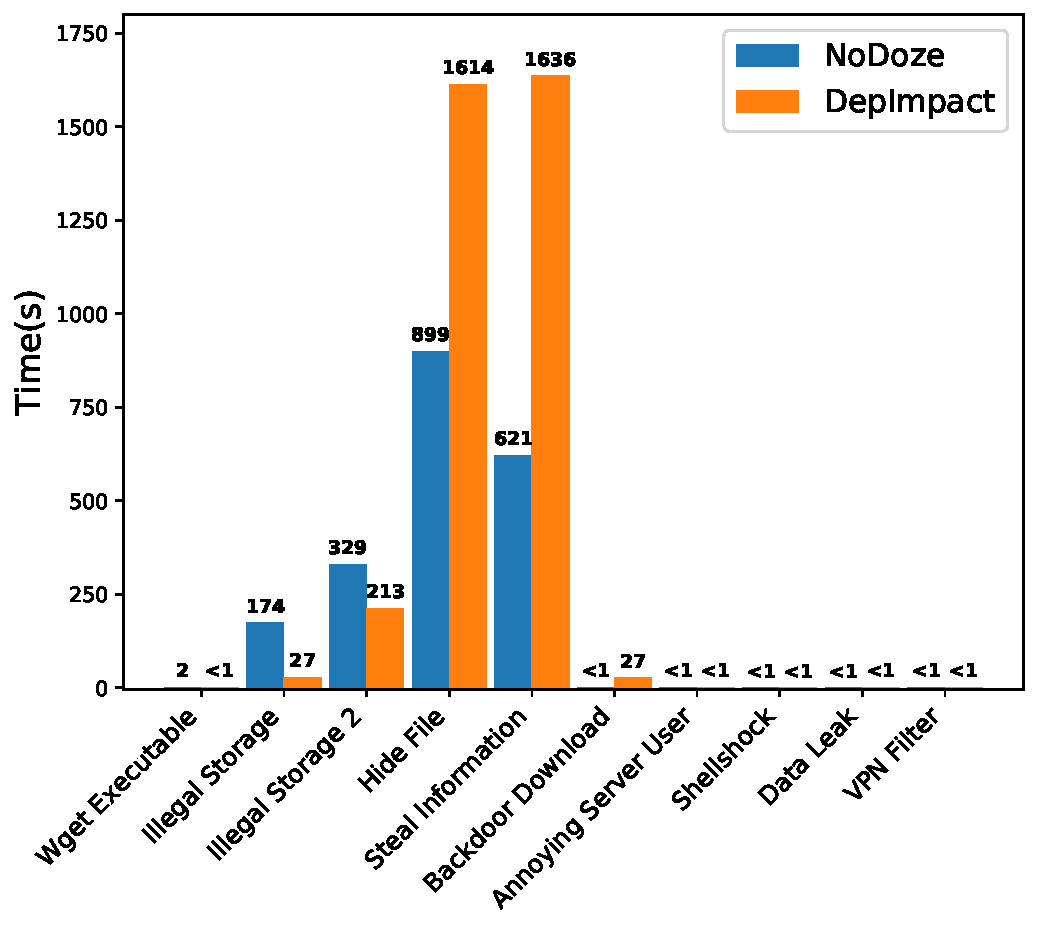
\includegraphics[width=0.48\textwidth]{figs/s&p/rq4.pdf}
    \caption{Runtime performance of \tool and NoDoze}
    \label{fig:rq4compare}
\end{figure}

\subsection{RQ4: System Performance}

To understand the performance of \tool, we measure the execution time of each step in \tool, as shown in \cref{tab:rq4performance}.
On average, \tool takes $430s$ to finish
%the processing and computation for one 
analyzing an attack, and dependency graph construction (\ie Causality Analysis) requires $69.98s$ and edge merge requires $8.56s$.
%
We compare \tool with the average-projection approach for dependency weight computation and dependency impact propagation, since they share the same steps for causality analysis and edge merge. 
From \cref{tab:rq4performance}, we observe that 
(1) \tool takes more time for dependency weight computation ($\sim102s$) because \tool uses the Multi-KMeans++ clustering and LDA to find the optimal projection vector;
(2) \tool takes less time for dependency impact propagation. The reason is because the dependency weights computed by \tool are much more discriminative, and hence the score propagation can converge faster.
%but the shorter time for the average-projection approach in dependency weight computation is offsetted by the time needed for score propagation. 
As a result, \tool reduces the execution time by $80.23\%$ when compared with the average-projection approach. 

We also compare the execution time of \tool (dependency weight computation plus dependency impact propagation) with the execution time of NoDoze (anomaly score computation), since they share the same causality analysis and edge merge steps.
\cref{fig:rq4compare} shows the results.
%
We observe that \tool is more efficient than NoDoze for 2 attacks (\ie the ``Illegal Storage'' attack and ``Illegal Storage 2'' attack), as efficient as NoDoze for 5 attacks, and less efficient for 3 attacks.
In particular, while \tool requires more time for processing the 2 attacks whose dependency graphs have more than 3 million edges (\ie the ``Hide File'' attack and the ``Steal information'' attack), \tool produces much smaller graphs ($\sim800$ edges) than NoDoze ($>20,000$ edges).
On average, \tool needs $351.8$s to finish the dependency weight computation and the dependency impact propagation, and NoDoze needs $202.65$s to finish the anomaly score computation ($430.34s$ v.s. $281.19s$ for the whole analysis).
%
Thus, \tool and NoDoze have similar runtime performance for most of the attacks, and NoDoze is more efficient for certain attacks at the cost of poor graph reduction. 



\eat{
Also, the results in \cref{subsec:rq3} show that \tool achieves better ranking for the attack entries than the average-projection approach, and we want to know whether it is at the cost of more computation efforts.
The results are shown in \cref{tab:rq4performance}.



To understand the performance of \tool in investigating real attacks, we measure the execution time of \tool on the attack cases.
\tool starts the computation by parsing a log ($92.252s$ averagely) and building a global graph representation ($3.277s$ averagely).
\cref{tab:runtime} shows the execution time for the remaining components of \tool. 
Besides the steps shown in the preprocessing step, \emph{Causality Analysis}, \emph{Edge Merge}, and \emph{Node split} require $0.21s$, $0.06s$, and $0.003$ on average. 
Note that \emph{Weight Computation} and \emph{Reputation Propagation} only requires $0.25s$ and $0.01s$ on average.
In summary, the total time for running an analysis is about $2$ minutes, but the major cost (\ie log parsing) can be improved by adopting caching or database indexing~\cite{gao2018aiql}.
}